\documentclass{article}[10pt]
\usepackage{float,amsmath}
\usepackage{graphicx}
\usepackage{color}
\usepackage[letterpaper,margin=1in]{geometry}
\usepackage{hyperref}

%\setlength{\textwidth}{6.5in}

\begin{document}

\author{David DeBoer}
\title{Array Configuration Management Database}
\maketitle

\section{Introduction}
The HERA array/part configuration management database is a set of five tables within the larger hera\_mc database, which is maintained on-site in the Karoo.  The tables are detailed in the Appendix, 
but they are: 

\begin{center}
\begin{tabular}{l l l}
         {\bf psql table} & {\bf in python file}  &  {\bf with class name} \\
	geo\_location 	& hera\_mc/geo\_location.py & GeoLocation \\
	station\_type 	& hera\_mc/geo\_location.py & StationType \\
	parts\_paper 	& hera\_mc/part\_connect.py & Parts \\
	part\_info 	         & hera\_mc/part\_connect.py & PartInfo \\
	connections 	& hera\_mc/part\_connect.py & Connections \\
\end{tabular}
\end{center}

Software is contained in the repository https://github.com/HERA-Team/hera\_mc.

The databases are structured primarily around {\em parts} and {\em connections}.  {\em Parts} are meant to be single items that, in theory at least, are a thing than can be replaced as a unit.  
{\em Connections} define {\em ports} on a given parts and connect two ports together.  Parts are all upper case and ports are all lower case.

All parts and connections are timed in that they have a start and stop time of operation.  If stop is {\tt None}, then it is active (it is given a date in the relatively far future).  There are currently two special parts (one at each end of the signal chain):
\begin{itemize}
	\item {\bf geo\_location}: a geo\_located part (``station'') is a named location with UTM coordinates which also has an entry in the geo\_location table;
	\item {\bf f\_engine}:  each input to the f\_engine ROACH-2 is currently listed as a separate part.  Probably it should be a 32-input part, but given timing will wait for the new architecture.
\end{itemize}

Parts are hooked together via connections of their ports.   For parts in the PAPER era, the signal chain hook-up is given below and shown in Fig. \ref{fig:hookup}.
\begin{itemize}\setlength\itemsep{-.3em}
	\item {\bf Station}: geo\_located position.  See prefixes in table station\_meta ({\em e.g.} {\tt HH} for herahex)
	\item {\bf Antenna\footnote{Note that rev {\bf P} is the PAPER element, {\bf T} is the transitional numbering, {\bf H} is HERA}}:  collecting element ({\em this is the correlator antenna number}):  {\tt{\bf A}}
	\item {\bf Feed}:  element feed.  {\tt {\bf FDP}\{\#\}} are PAPER feeds, {\tt {\bf FDA}\{\#\}} are design A HERA feeds.
	\item {\bf Front-end}:  lna, etc at feed.  {\tt {\bf FEA}\{\#\}} is design A (75 $\Omega$, NRAO).  {\tt {\bf FEM}\{\#\}} is the 75 $\Omega$, CAM).
	\item {\bf Cable-feed75}:  cable from front-end to receiverator: {\tt {\bf C7F}\{\#\}}
	\item {\bf Cable-post-amp(in)}:  cable inside {\tt R}$^{th}$ receiverator to post-amp: {\tt {\bf RI}\{R\}\{"A"/"B"\}\{\#\}\{"E"/"N"\}}
	\item {\bf Post-amp}:  post-amp in receiverator: {\tt {\bf RCVR}\{\#\}} (75 $\Omega$, NRAO).  {\tt {\bf PAM}\{\#\}} is the 75 $\Omega$, CAM).
	\item {\bf Cable-post-amp(out)}:  cable inside receiverator from post-amp {\tt {\bf RO}\{R\}\{"A"/"B"\}\{\#\}\{"E"/"N"\}}
	\item {\bf Cable\_receiverator}:  cable from receiverator to container {\tt {\bf CR}\{R\}\{"A"/"B"\}\{\#\}\{"E"/"N"\}}
	\item {\bf Cable\_container}:  cable inside container from {\tt\{P\}}late/{\tt\{Row\}}/{\tt\{Col\}}umn {\tt {\bf CC}\{P\}{\bf R}\{Row\}{\bf C}\{Col\}}
	\item {\bf F-engine}:  {\tt\{R2\}} Roach-2 input {\tt {\bf DF}\{R2\}\{"A"-"H"\}\{\#\}}
\end{itemize}
The {\tt E} and {\tt N} refer to the polarizations (for East and North) -- this replaces any X/Y or H/V designation.
Summarizing with prefixes, we have 

\vspace{.15in}
\begin{center}
{\tt HH-A-FD-FE-C7F-RI-RCVR-RO-CR-CC-DF}
\end{center}
\vspace{.15in}

\begin{figure}[H]
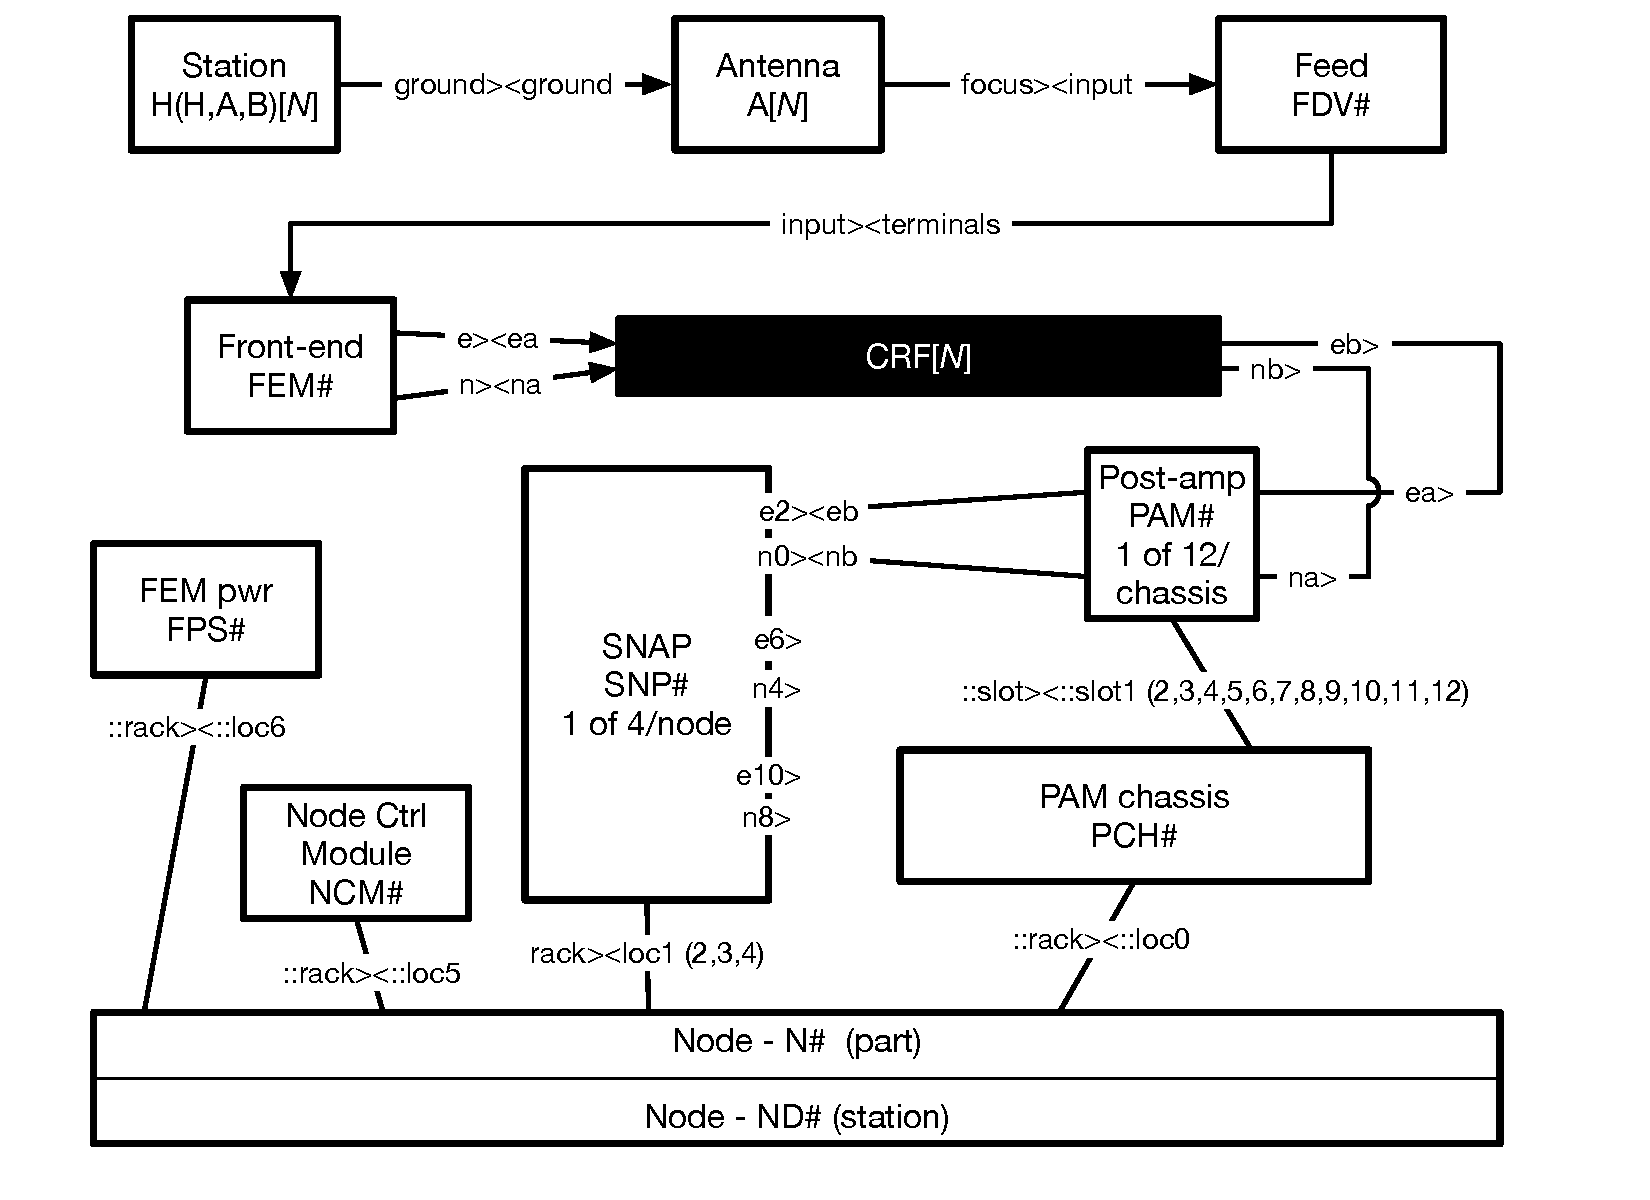
\includegraphics[width=0.8\textwidth]{hookup.pdf}
\centering
\caption{Block diagram of hookup.  Filled boxes are cables, blue objects are in the receiverator and green objects are in the container.
The line labels indicate the port names/connections.}
\label{fig:hookup}
\end{figure}

\section{Package Modules}
This section provides a high-level overview of the python configuration management package modules within hera\_mc that are called from scripts or used in interactive sessions.
\vspace{0.5cm}

\begin{tabular}{l p{12cm}}
{\bf geo\_location.py} & Defines {\tt station\_type} and {\tt geo\_location}.  Provides update utility for {\tt geo\_location}.  Contains {\tt is\_in\_geo\_location} and {\tt is\_in\_connections}. \\ \hline
{\bf geo\_handling.py} & Contains myriad defs that handle various geo functionalities.\\ \hline
{\bf part\_connect.py} & Defines {\tt parts\_paper}, {\tt part\_info}, and {\tt connections}.  Provides update utilities for {\tt parts\_paper} and {\tt connections}. Contains {\tt \_\_get\_part\_revisions}. \\ \hline
{\bf cm\_table\_info.py} & Has mapping and order of tables and classes for initialization. \\ \hline
{\bf cm\_handling.py} & Defines the {\tt Handling} class to handle various configuration management functionalities.\\ \hline
{\bf cm\_transfer.py} & Contains myriad defs that help package and initialize the cm tables.\\ \hline
{\bf cm\_part\_revisions.py} & Contains myriad defs that deal with finding revision numbers etc.\\ \hline
{\bf cm\_hookup.py} & Defines the {\tt Hookup} class to help determine and show the full part hookup.\\ \hline
{\bf cm\_dataview.py} & Contains various methods to display cm information.\\ \hline
{\bf cm\_utils.py} & Contains various defs called by other modules.\\
\end{tabular}

\section{Scripts}
This section provides a high-level overview of the high-level scripts:  geo.py, parts.py, cmdv.py.  Note that info you type {\tt info} after them, it presents information on them.  The structure is 

{\tt geo.py {\it action} --arguments}

\noindent {\tt {\it action} } is optional with a default.

\subsection{geo.py}
Has various plotting/printing options for station information.  Available actions are (note you need the first 3 letters only):

\begin{itemize}
\item {\tt geo} [default]:  plots and/or lists ({\tt -g}) antenna locations.  Plots have the "background" behind them.
\item {\tt cofa}:  plots and/or lists the position of the center of the array.
\item {\tt since}:  plots and/or lists the antennas built since the provided date.
\item {\tt info}:  provides information on the script.
\end{itemize}

{\tt geo.py -g -l HH67} will show the "background" (selectable via --station-types or -t) of active (selectable via --show-state) antennas with HH67 highlighted.  It will provide an overview printout as well.

\subsection{parts.py}
Has various printing options for part information (part info, connections, hookup, types, etc).  Available actions are (note you only need the first 2 letters only):

\begin{itemize}
\item {\tt hookup} [default]:  lists hookup info for parts (as a csv list with no spaces) after -p
\item {\tt part\_info}:   provides a summary of given part(s)
\item {\tt conn\_info}:   provides a summary table of parts connected to given part(s)
\item {\tt rev\_info}:  provides a summary of revisions to given part(s)
\item {\tt types}:  prints a summary table of part types
\item {\tt check\_rev}:  checks whether a given revision of a part exists
\item {\tt overlap\_check}:  checks that the given part doesn't have overlapping revisions.
\item {\tt info}:   provides information on the script
\end{itemize}

{\tt parts.py -p ri5} will provide a table of all hookups to receiverator 5.  {\tt parts.py -p ri5 --hookup-cols "station,cable-post-amp(in),f-engine"}  will just show those columns.

\subsection{cmdv.py}
Has various plotting/printing options for correlator and general information.  Available actions are (note you need the first 2 letters only):

\begin{itemize}
\item {\tt corr} [default]:  Provides information on the correlator hookups for the supplied --date/--time.
\item {\tt fc-view}:  fully-connected view of part --parts(-p) between date and date2.
\item {\tt file-view}:  plot the supplied fc-view files
\item {\tt info}:  provides information on the script.
\end{itemize}

{\tt cmdv.py} will provide all of the current station-correlator pairings

\section{Use Cases}
Three use cases are identified:
\begin{enumerate}\setlength\itemsep{-.3em}
	\item In-the-field
	\item Remote user
	\item Bulk database
\end{enumerate}

\subsection{In-the-field updates}
This is the ``operational'' mode, where inputs to the on-site database are done via scripts (command-line and/or web), which update the database directly.  These scripts will be documented under the repository software.

\subsection{Remote user}
Remote use is the case when a remote user initializes and uses the tables outside of the main database.  This assumes that postgresql etc is configured on the remote computer.  Note that this mode supports both offline use (essentially steps 3-5 below, which are in bold) and development (probably all steps).  The process is as follows: 
\begin{enumerate}\setlength\itemsep{-.3em}
	\item Generate ascii files of the tables in the main database (in the Karoo) {\tt (cm\_pack.py [--tables table1,table2,...)}
	\item Push to GitHub
	\item {\bf Pull down to remote computer}
	\item {\bf Install ({\tt python setup.py install})}
	\item {\bf Initialize the updated ones ({\tt cm\_init.py})}
	\item If you are developing, make a base version before you start ({\tt cm\_pack.py --base})
\end{enumerate}

Note that generally you should leave off the {\tt --tables} option, since you should use all the tables so as to not break foreign keys (it is left there for ``expert'' users).  Steps 3-5 are bolded, since if you just want to pull down the latest and use it assuming things are up-to-date they are all that are needed (i.e., leave the ``packaging to the experts'').

This has another option of {\tt --base}, so that you can set up a base copy to which you can revert if need be by including {\tt --base} on both commands (step 6).
	
\subsection{Main database updates}
This is effectively the opposite of the remote user case, bringing an updated set of table(s) back into the main database.  The process is as follows:
\begin{enumerate}\setlength\itemsep{-.3em}
	\item  Generate ascii files of the desired tables from the remote database: 
		({\tt cm\_pack.py --maindb \$key [--tables table1,table2,...]})
	\item Push to GitHub
	\item Pull down to site computer
	\item Install
	\item Update existing tables  ({\tt cm\_init.py --maindb \$key [--tables table1,table2,]})
\end{enumerate}

Note that {\tt \$key} is a user supplied string to just make sure you meant to do the main database update.  It can be anything, you
just need to remember it when you reload it on the main database computer qmaster.
As per above, you should generally leave off the {\tt --tables} option so as to do them all.  

\section{Tables}
As mentioned above, there are five tables in the configuration management section of the database:  (1) geo\_location, (2) station\_meta,
(3) parts\_paper, (4) part\_info, (5) connections.  The following tables summarize them with the following key:  
\begin{itemize}\setlength\itemsep{-.3em}
	\item {\bf Bold font} = primary key
	\item {\em Italics} = foreign\_key.
	\item * = NotNull entries
\end{itemize}

\begin{table}[h]
\centering
\caption{geo\_location :: geo\_location.GeoLocation}
\begin{tabular}{| l | l | l |} \hline
{\bf Column} & {\bf Type} & {\bf Description} \\ \hline
{\bf station\_name}*  & character varying(64) & Name of position - never changes \\ \hline
{\em station\_type\_name}* & character varying(64) & Type of station \\ \hline
datum & character varying(64) & UTM datum \\ \hline
tile & character varying(64) & UTM tile \\ \hline
northing & double precision & UTM coordinate \\ \hline
easting & double precision & UTM coordinate \\ \hline
elevation & double precision & Elevation \\ \hline
created\_gpstime* & BigInt & GPS second of creation. \\ \hline
\end{tabular}
\end{table}

\begin{table}[h]
\centering
\caption{geo\_location :: station\_type.StationType}
\begin{tabular}{| l | l | l |} \hline
{\bf Column} & {\bf Type} & {\bf Description} \\ \hline
{\bf \em station\_type\_name}* &  character varying(64) &  Station type name \\ \hline
prefix* & character varying(64) & 1-2 letter prefix for part station\_name \\ \hline
description & character varying(64) &  Short description \\ \hline
plot\_marker & character varying(64) & Type of matplotlib marker \\ \hline
\end{tabular}
\end{table}

\begin{table}[h]
\centering
\caption{part\_connect :: parts\_paper.Parts}
\begin{tabular}{| l | l | l |} \hline
{\bf Column} & {\bf Type} & {\bf Description} \\ \hline
{\bf \em hpn}* & character varying(64) & HERA part number \\ \hline
{\bf \em hpn\_rev}* & character varying(32) & HPN revision letter (A-Z) \\ \hline
hptype*  &  character varying(64) & HPN part type category \\ \hline
manufacturer\_number & character varying(64) & Unique serial number for each part \\ \hline
start\_gpstime* & BigInt & GPS second when part/rev is activated. \\ \hline
stop\_gpstime & BigInt & GPS second when part/rev is de-activated \\ \hline
\end{tabular}
\end{table}

\begin{table}[h]
\centering
\caption{part\_connect :: part\_info.PartInfo}
\begin{tabular}{| l | l | l |} \hline
{\bf Column} & {\bf Type} & {\bf Description} \\ \hline
{\bf \em hpn}* & character varying(64) & HERA part number \\ \hline
{\bf \em hpn\_rev}* & character varying(32) & HPN revision letter (A-Z) \\ \hline
posting\_gpstime* & BigInt & GPS second information was posted \\ \hline
comment* &  character varying(1024) & Comment \\ \hline
library\_file & character varying(256) &  Librarian filename (how to get it there?) \\ \hline
\end{tabular}
\end{table}

\begin{table}[h]
\centering
\caption{part\_connect :: connections.Connections}
\begin{tabular}{| l | l | l |} \hline
{\bf Column} & {\bf Type} & {\bf Description} \\ \hline
{\bf \em upstream\_part}* &  character varying(64) & Hera part number of upstream connection \\ \hline
{\bf \em up\_part\_rev}* & character varying(32) & Hera part revision of upstream connection \\ \hline
{\bf upstream\_output\_port}* & character varying(64) & Output port on upstream part \\ \hline
{\bf \em downstream\_part}* & character varying(64) & Hera part number of downstream connection \\ \hline
{\bf \em down\_part\_rev}* & character varying(32) & Hera part revision of downstream connection \\ \hline
{\bf downstream\_input\_port}* & character varying(64) & Input port on downstream part \\ \hline
{\bf \em start\_gpstime}* & BigInt & GPS second when connection started \\ \hline
stop\_gpstime & BigInt & GPS second when connection ended \\ \hline
\end{tabular}
\end{table}

\end{document}